% fs-02-ElementaryProbability.tex

\documentclass[xcolor=dvipsnames]{beamer}

\usepackage{graphicx}
\usepackage{wrapfig}
\usepackage{colortbl}
\usepackage{alltt}
\definecolor{myblue}{rgb}{0.8,0.85,1}

\mode<presentation>
{
  \usetheme{Warsaw}
  \setbeamercovered{transparent}
}
% \usecolortheme[named=OliveGreen]{structure}
\setbeamertemplate{navigation symbols}{} 
\setbeamertemplate{blocks}[rounded][shadow=true] 

\newif\ifBCITCourse
\BCITCoursetrue
% \BCITCoursefalse
\newif\ifWhichCourse
\WhichCoursetrue
% \WhichCoursefalse
\ifBCITCourse
\ifWhichCourse
\newcommand{\CourseName}{Statistics for Food Technology}
\newcommand{\CourseNumber}{MATH 2441}
\newcommand{\CourseInst}{BCIT}
\else
\newcommand{\CourseName}{Calculus for Geomatics}
\newcommand{\CourseNumber}{MATH 2511}
\newcommand{\CourseInst}{BCIT}
\fi
\else
\newcommand{\CourseName}{Philosophy and Literature}
\newcommand{\CourseNumber}{PHIL 375}
\newcommand{\CourseInst}{UBC}
\fi

\title{Elementary Probability}
\subtitle{{\CourseNumber}, BCIT}

\author{\CourseName}

\date{January 8, 2018}

% \begin{figure}[h]
% 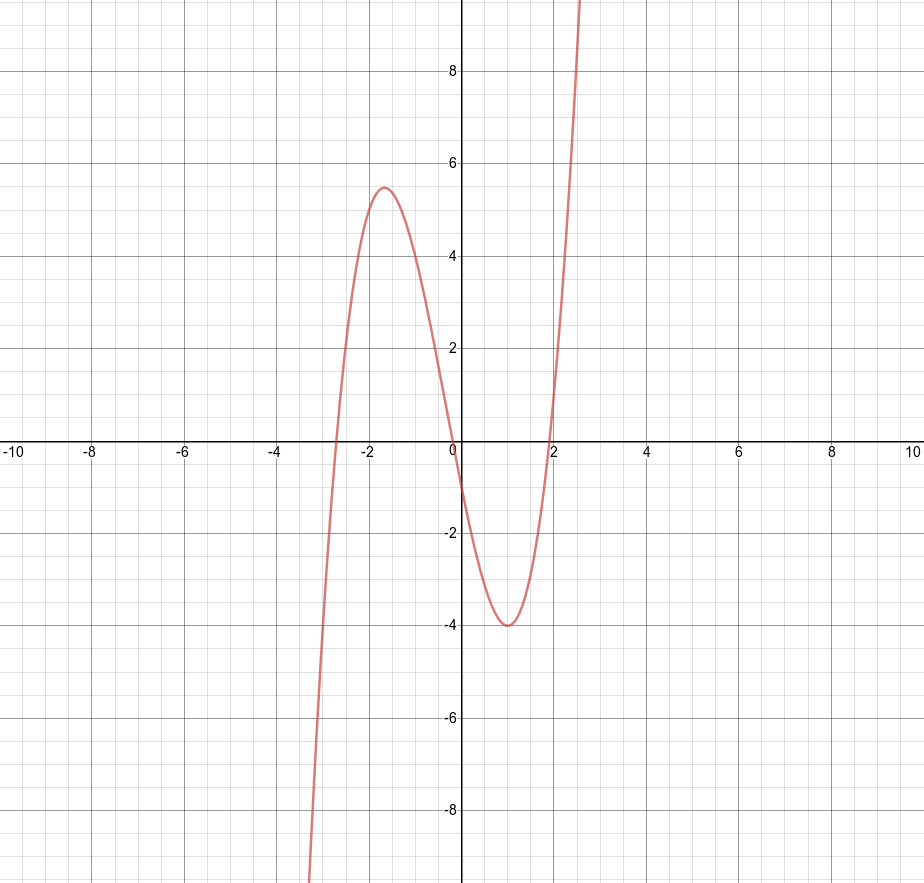
\includegraphics[scale=.3]{./extrema1.png}
% \end{figure}

% Command             10pt    11pt    12pt
% \tiny               5       6       6
% \scriptsize         7       8       8
% \footnotesize       8       9       10
% \small              9       10      10.95
% \normalsize         10      10.95   12

\begin{document}

\begin{frame}
  \titlepage
\end{frame}

\begin{frame}
  \frametitle{Definitions}
  \begin{description}
  \item[event] An event is any collection of results or outcomes of a
    procedure.
  \item[sample space] The sample space for a procedure consists of all
    possible simple events. That is, the sample space consists of all
    outcomes that cannot be broken down any further. The symbol for
    the sample space is $\Omega$. 
  \item[complement] The complement of event $A$ is $\urcorner{}A$ and
    consists of all outcomes in which $A$ does not occur.
  \end{description}
\end{frame}

\begin{frame}
  \frametitle{Logic and Sets I}
  \begin{enumerate}
  \item<1-> $A\vee{}B$ is the event ``either $A$ or $B$ happens.''
  \item<2-> $A\wedge{}B$ is the event ``both $A$ and $B$ happens.''
  \item<3-> $\urcorner{}A$ is the event ``$A$ does not happens.''
  \item<4-> $\Omega$ and $\emptyset$ are events; they are called
    `tautology' and `contradiction,' respectively.
  \end{enumerate}
\end{frame}

\begin{frame}
  \frametitle{Logic and Sets II}
  The logical statement $A\vee{}B$ corresponds to the union of sets
  $A\cup{}B$ if $A$ and $B$ are understood as sets of simple events.

\medskip

  The logical statement $A\wedge{}B$ corresponds to the intersection of sets
  $A\cap{}B$ if $A$ and $B$ are understood as sets of simple events.

\medskip

Events $A$ and $B$ are \alert{disjoint} (or \alert{mutually
  exclusive}) if they cannot occur together. In set theory, we can
express this by saying that they are disjoint if and only if
$A\cap{}B=\emptyset$.

Think of dice rolls as an example. $\Omega=\{1,2,3,4,5,6\}$. Event $A$
may be $\{1,2,3\}$, and event $B$ may be $\{2,4,6\}$. What, then, are
events $A\cup{}B$ and $A\cap{}B$?
\end{frame}

\begin{frame}
  \frametitle{Definition of Probability}
Let $\Omega$ be a set of simple events. An event $A$ is then a subset
of $\Omega$. A function $P$ from the collection of all these subsets
(sometimes called the power set of $\Omega$) to the real numbers is a
\alert{probability function} if the following three conditions are
fulfilled.
\begin{enumerate}
\item<1-> $P(A)\geq{}0$ for all events $A$.
\item<2-> $P(\Omega)=1$.
\item<3->
  $P(A_{1}\cup{}A_{2}\cup\ldots\cup{}A_{n})=P(A_{1})+P(A_{2})+\ldots{}+P(A_{n})$
  for any collection of disjoint events $A_{1},A_{2},\ldots,A_{n}$.
\end{enumerate}
\end{frame}

\begin{frame}
  \frametitle{Basic Theorems of Probability}
Here are some basic theorems that follow from the conditions.
\begin{block}{Rule of Complementary Events}
  $P(\urcorner{}A)=1-P(A)$\mbox{ for all events }A
\end{block}
This immediately implies that $P(\emptyset)=0$ since
$\emptyset=\urcorner\Omega$.
\begin{block}{Addition Rule}
  $P(A\cup{}B)=P(A)+P(B)-P(A\cap{}B)$
\end{block}
\end{frame}

\begin{frame}
  \frametitle{Conditional Probability}
Conditional probability of $A$ conditional on $B$ is defined as follows,
\begin{equation}
  \label{eq:iekeengi}
  P(A|B)=\frac{P(A\cap{}B)}{P(B)}
\end{equation}
This theorem follows immediately,
\begin{block}{Multiplication Rule}
  $P(A\cap{}B)=P(A)\cdot{}P(B|A)$
\end{block}
Two events $A$ and $B$ are \alert{independent} if and only if
$P(A\cap{}B)=P(A)\cdot{}P(B)$. Given the multiplication rule, this is
equivalent to saying that $P(A|B)=P(A)$ and $P(B|A)P(B)$.
\end{frame}

\begin{frame}
  \frametitle{Exercises I}
  \begin{block}{Always remember {\ldots}}
  {\ldots} when $A$ and $B$ are \emph{disjoint}, then
  $P(A\cup{}B)=P(A)+P(B)$; when $A$ and $B$ are \emph{independent},
  then $P(A\cap{}B)=P(A)\cdot{}P(B)$.
  \end{block}
\textbf{Exercise 0.} Your friend tosses two coins. You don't see the
coins, but your friend tells you that at least one of them landed
heads. What is the probability that they both landed heads?

\textbf{Exercise 1.} Alice has brown eyes. Branden has blue eyes. Their son
Joel has blue eyes. What is the probability that their next child will
have blue eyes as well?

\textbf{Exercise 2.} In a sample of 207 adults, 43 are smokers. What
is the probability of choosing a person at random who is a smoker?
\end{frame}

\begin{frame}
  \frametitle{Exercises II}
\textbf{Exercise 3.} A game show host asks you a multiple choice
question with four answers A, B, C, and D. If you make a random guess,
what is your probability of getting the correct answer?

\textbf{Exercise 4.} In a country far away, all parents want to have
girls. The probability of having a girl is 50\%. All parents have boys
until they have a girl. What would you expect to be the proportion of
girls in that country?

\textbf{Exercise 5.} The government found out that 102 out of 810
luggage scales at the airport are defective. If you choose 2 luggage
scales at random \emph{with replacement}, what is the probability that
they are both defective? If you choose 2 luggage scales at random
\emph{without replacement}, what is the probability that they are both
defective?
\end{frame}

\begin{frame}
  \frametitle{Tree Diagrams I}
\textbf{Exercise 6.} The probability that BCIT hires a person on a
particular weekday is the same as any other weekday. What is the
probability that two randomly selected employees were both hired on a
Monday? What is the probability that two randomly selected employees
were both hired on the same weekday?

\textbf{Exercise 7.} In a group of people, 492 would choose a window
seat on an airplane, 8 would choose a middle seat, and 306 would
choose an aisle seat. What is the probability of randomly choosing a
person who would not choose a middle seat? What is the probability of
randomly choosing two people who would not choose a middle seat? What
is the probability of randomly choosing twenty-five people who would
not choose a middle seat?
\end{frame}

\begin{frame}
  \frametitle{Tree Diagrams II}
\textbf{Exercise 8.} What is the probability of rolling a sum of 9 on
two dice rolls?

\textbf{Exercise 9.} What is the probability of having two girls and
three boys when there are five children and the probability of having
a boy is 50\%?
\end{frame}

\begin{frame}
  \frametitle{Tree Diagrams}
You can use independence and mutual exclusion to draw tree diagrams.
\begin{figure}[h]
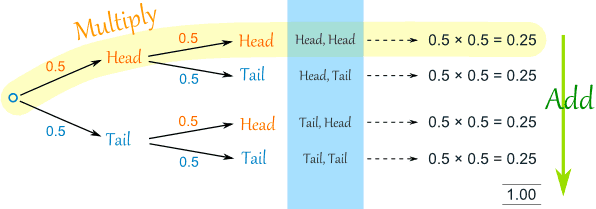
\includegraphics[scale=.5]{./tree.png}
\end{figure}
\end{frame}

\begin{frame}
  \frametitle{Exercise Tree Diagram}
\textbf{Exercise 10.} You have two coaches, Sam and Alex. When Sam
coaches the team, your proability of being the goalkeeper is 50\%. When Alex
coaches the team, your proability of being the goalkeeper is 30\%. The
probability that Sam (rather than Alex) will coach your team today is
60\%. What is the probability that you will be goalkeeper?
\end{frame}

\newcommand{\sam}{.65}

\begin{frame}
  \frametitle{Sam and Alex I}
\begin{figure}[h]
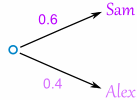
\includegraphics[scale=\sam]{./sam1.png}
\end{figure}
\end{frame}

\begin{frame}
  \frametitle{Sam and Alex II}
\begin{figure}[h]
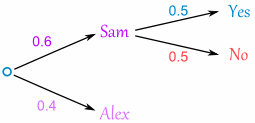
\includegraphics[scale=\sam]{./sam2.png}
\end{figure}
\end{frame}

\begin{frame}
  \frametitle{Sam and Alex III}
\begin{figure}[h]
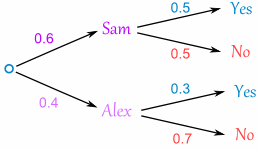
\includegraphics[scale=\sam]{./sam3.png}
\end{figure}
\end{frame}

\begin{frame}
  \frametitle{Sam and Alex IV}
\begin{figure}[h]
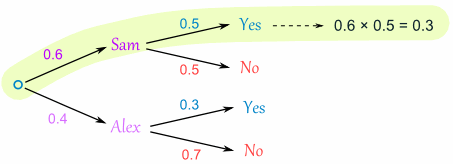
\includegraphics[scale=\sam]{./sam4.png}
\end{figure}
\end{frame}

\begin{frame}
  \frametitle{Sam and Alex V}
\begin{figure}[h]
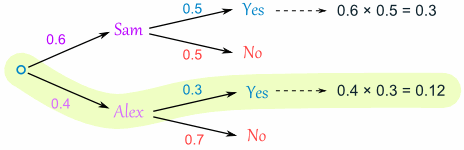
\includegraphics[scale=\sam]{./sam5.png}
\end{figure}
\end{frame}

\begin{frame}
  \frametitle{Sam and Alex VI}
\begin{figure}[h]
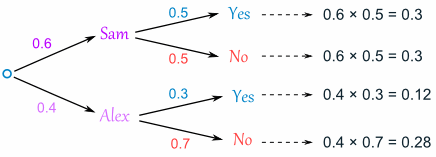
\includegraphics[scale=\sam]{./sam6.png}
\end{figure}
\end{frame}

\begin{frame}
  \frametitle{How to Solve Probability Problems}
In summary, here are some strategies to solve probability problems.
\begin{enumerate}
\item<1-> Count simple events. If the simple events are all equally
  probable, then the probability of event $A$ is the number of simple
  events in $A$ divided by the total number of simple events, so
  $P(A)=\#A/\#\Omega$.
\item<2-> Make sure to watch for independence and mutual exclusion.
  Whenever events are independent or mutually exclusive (disjoint),
  you can use $P(A\cap{}B)=P(A)P(B)$ or $P(A\cup{}B)=P(A)+P(B)$,
  respectively.
\item<3-> If events are not mutually exclusive, you can use the
  addition rule $P(A\cup{}B)=P(A)+P(B)-P(A\cap{}B)$.
\item<4-> If events are not independent, you can use conditional
  probabilities in $P(A\cap{}B)=P(A)P(B|A)$.
\item<5-> If you are dealing with events that are independent and
  mutually exclusive, it is often useful to draw a tree diagram.
\end{enumerate}
\end{frame}

\begin{frame}
  \frametitle{End of Lesson}
Next Lesson: Counting.
\end{frame}

\end{document}
